\documentclass[a4paper]{article}

%% Language and font encodings
\usepackage[english]{babel}
\usepackage[utf8x]{inputenc}
\usepackage[T1]{fontenc}

%% Sets page size and margins
\usepackage[a4paper,top=3cm,bottom=2cm,left=3cm,right=3cm,marginparwidth=1.75cm]{geometry}

%% Useful packages
\usepackage{amsmath}
\usepackage{graphicx}
\usepackage[colorinlistoftodos]{todonotes}
\usepackage[colorlinks=true, allcolors=blue]{hyperref}

\title{Most popular completion math QAC report}
\author{Wei Zhong}

\begin{document}
\maketitle

\begin{figure}
\centering
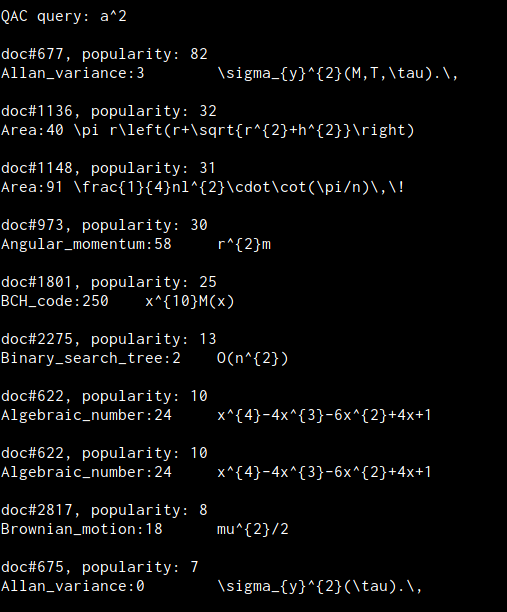
\includegraphics[width=0.5\textwidth]{qac-results.png}
\caption{\label{fig:qac}QAC results based most popular completion for query $a^2$}
\end{figure}

\section{Introduction}

Query autocompletion is widely adopting ``most popular completion" (MPC) method \cite{Bar-Yossef:2011} to suggest query completion and it is the baseline method used to compare other query autocompletion results in many research papers. Most popular completion is a method to prioritize query autocompletion suggestions based on the frequency the candidate query has appeared in query log (usually a search engine maintained log that records user query history). Here we describe the algorithm and implementation of query autocompletion based on frequency for math search, apply MPC into math-aware search query auto completion, and test a few formula query by using MPC method.

\section{Implementation}
In normal text search engine, query frequency is measured by how many times an unique query has been observed in query log \cite{cai_survey_2016}. However, it is unclear how we measure the uniqueness of a math query, since math expression can have associativity and commutativity, if we do not take the structure variance into account, query completion results for a math expression is likely to give duplicated expression results with same math semantic meaning.
To count the frequency of math formula, we need to define the uniqueness of a math expression. Based on our previous method which evaluate math expression structure similarity by decomposing math semantic operator tree into leaf-root paths, here we define the uniqueness of math expression by the set of leaf-root paths it generates.

The method can be divided into two stages, in index stage, document math expressions are indexed in such a way that only an ``unseen" (by the definition of our uniqueness) expression is indexed, and its frequency in query log is initially set to one (frequency value is stored in a key-value database where its value is mapped to an expression ID assigned to this expression). Later if the same expression is appended into query log, we find its corresponding identical expression in our index, and get the identical expression ID through merging the corresponding posting lists of its leaf-root path set. After unique expression ID is obtained, we update the frequency in the key-value database.

The index procedure is scratched as follows,
\begin{verbatim}
Function index(tex)
    result := math_expr_search(tex);
    if result is not empty:
        key_value_db[result[0].exprID].freq += 1
    else:
        operator_tree := parse(tex)
        if no parser error reported:
            cur_len = len(key_value_db)
            new_exprID = cur_len + 1
            key_value_db[new_exprID].freq = 1
            Index math expression structure
\end{verbatim}

Later, if a query is entered, we search for the math expression index and find any expressions matches either exactly to the query or having the query expression being a sub-expression, if any such document expression is found, we retrieval the expression as well as the frequency value it associates (from key-value database) and rank the suggested expressions by their frequency.

\section{Experiment}
To start experience math query autocompletion by query log frequency without judgement data, I try to use a faked small dataset to produce some preliminary results. I use a ~10K size expressions from a subset of NTCIR-12 corpus to index them as faked query log. The resulting unique math expressions is around 3400. Here are some example queries and their query suggestions by popularity (see Figure~\ref{fig:qac} for example output):

\begin{center}
\begin{tabular}{lc}
Suggesions $\backslash$ Query  & $x^2$ \\
\hline
 1 & $\sigma_{y}^{2}(M,T,\tau)$ \\
 2 &  $\pi r\left(r+\sqrt{r^{2}+h^{2}}\right)$ \\
 3 & $\frac{1}{4}nl^{2}\cdot\cot(\pi/n)\,\! $ \\
 4 & $r^{2}m$ \\
 5 & $x^{10}M(x)$ \\
 6 & $O(n^{2})$ \\
\end{tabular}
\end{center}

\begin{center}
\begin{tabular}{lc}
Suggesions $\backslash$ Query  & $x^2 + $ \\
\hline
 1 &  $\pi r\left(r+\sqrt{r^{2}+h^{2}}\right)$ \\
 2 &  $ f(x)=\frac{1}{x^{2}+1} $\\
 3 & $ S(x)=\alpha^{4}+\alpha^{-7}x+\alpha^{1}x^{2}+ ...$ \\
 4 & $ m_{1}(x)=m_{2}(x)=m_{4}(x)=x^{4}+x+1,\, $  \\
 5 & $ \left[\frac{1}{2}(n^{2}+n)\right]T_{6}+\left[\frac{1}{2}(n^{2}+3n)\right]
T_{5} +(n+1)T_{4}+T_{1}+T_{2}+T_{3}+T_{7}\leq cn^{2},\ n\geq n_{0} $ \\
 6 & $   A\;=\;2\int_{-r}^{r}\sqrt{r^{2}-x^{2}}\,dx\;=\;\pi r^{2}     $ \\
 7 & $ (x+y)^{4}\;=\;x^{4}\,+\,4x^{3}y\,+\,6x^{2}y^{2}\,+\,4xy^{3}\,+\,y^{4} $ \\
 8 & $ x^{2}+y^{2}=1 $ \\
\end{tabular}
\end{center}

\begin{center}
\begin{tabular}{lc}
Suggesions $\backslash$ Query  & $x^2 + y$ \\
\hline
 1 & $ \left[\frac{1}{2}(n^{2}+n)\right]T_{6}+\left[\frac{1}{2}(n^{2}+3n)\right]
T_{5} +(n+1)T_{4}+T_{1}+T_{2}+T_{3}+T_{7}\leq cn^{2},\ n\geq n_{0} $ \\
 2 &  $ m_{1}(x)=m_{2}(x)=m_{4}(x)=x^{4}+x+1,\, $\\
 3 & $ g(x)=m_{1}(x)=x^{4}+x+1.\, $ \\
 4 & $ \sum_{k=0}^{n}k^{2}{\textstyle\left({{n}\atop{k}}\right)}=(n+n^{2})2^{n-2}  $  \\
 5 & $ \int 2x\,dx=x^{2}+C. $ \\
\end{tabular}
\end{center}

\bibliographystyle{alpha}
\bibliography{sample}

\end{document}
